\documentclass{include/thesisclass3}

\SelectLanguage{ngerman}
\usepackage{float}


% Titlepage settings
\newcommand{\praktikum}{Praktikum moderne Physik}
\newcommand{\autora}{Jens Schäfer}
\newcommand{\autorb}{Jan van der Linden}
\newcommand{\maila}{ugecd@student.kit.edu}
\newcommand{\mailb}{jan.vdlinden95@gmail.com}
\newcommand{\topic}{Spezifische Wärme}
\newcommand{\ptime}{10. Juli 2017}


% Shortcuts
\newcommand{\cc}{\cdot}
\newcommand{\rk}{\rangle}
\newcommand{\lk}{\langle}
\newcommand{\df}{\rightarrow}
\newcommand{\la}{\lambda}
\newcommand{\dd}{\text{d}}
\newcommand{\ehm}{\mathbbm{1}}
\newcommand{\p}{\partial}
\newcommand{\soll}{\overset{!}{=}}
\newcommand{\D}{\Delta}
\newcommand{\eps}{\epsilon}
\newcommand{\vektor}[3]{\begin{pmatrix} #1 \\ #2 \\ #3 \end{pmatrix}}
\newcommand{\vektorz}[2]{\begin{pmatrix} #1 \\ #2 \end{pmatrix}}
\newcommand{\Mat}[9]{\begin{pmatrix}#1&#2&#3\\#4&#5&#6\\#7&#8&#9\end{pmatrix}}
\newcommand{\Matz}[4]{\begin{pmatrix}#1&#2\\#3&#4\end{pmatrix}}
\newcommand{\e}[1]{\,\si{#1}}
\newcommand{\del}{\delta}
 


\begin{document}

	\FrontMatter
	% coordinates for background border
\newcommand{\diameter}{20}
\newcommand{\xone}{-15}
\newcommand{\xtwo}{160}
\newcommand{\yone}{15}
\newcommand{\ytwo}{-253}




\begin{titlepage}
    % background border
    \begin{tikzpicture}[overlay]
    \draw[color=gray]
            (\xone mm, \yone mm)
      -- (\xtwo mm, \yone mm)
    arc (90:0:\diameter pt)
      -- (\xtwo mm + \diameter pt , \ytwo mm)
        -- (\xone mm + \diameter pt , \ytwo mm)
    arc (270:180:\diameter pt)
        -- (\xone mm, \yone mm);
    \end{tikzpicture}



    % KIT image and sign for faculty of physics
    \begin{textblock}{10}[0,0](4.5,2.5)
        
\includegraphics[width=.25\textwidth]{include/kitlogo.pdf}
    \end{textblock}
    

    % horizontal line
    \begin{textblock}{10}[0,0](4.2,3.1)
        \begin{tikzpicture}[overlay]
        \draw[color=gray]
                (\xone mm + 5 mm, -12 mm)
          -- (\xtwo mm + \diameter pt - 5 mm, -12 mm);
        \end{tikzpicture}
    \end{textblock}



    % begin of text part
    \changefont{phv}{m}{n}    % helvetica
    \centering



    % thesis topic (en and ge)
    \vspace*{3cm}
    \Huge\praktikum\\



    % author name and institute
    \vspace*{5cm}
    
    \huge\topic\\






    % examiners (Referenten)
    \vspace*{3cm}
    \Large
    \begin{center}
        \begin{tabular}[ht]{l c l } 
  \autora & \hfill & \textit{\maila} \\
\autorb & \hfill & \textit{\mailb} \\
        
        \end{tabular}
    \end{center}



    % working time
    \vspace{2cm}
    \begin{center}
        \large{Durchgeführt am}: \ptime
    \end{center}



    % lowest text blocks concerning the KIT
    \begin{textblock}{10}[0,0](4,16.8)
        \tiny{KIT -- Universität des Landes Baden-Württemberg und nationales %
              Forschungszentrum in der Helmholtz-Gemeinschaft}
    \end{textblock}
    \begin{textblock}{10}[0,0](14,16.75)
        \large{\textbf{www.kit.edu}}
    \end{textblock}
\end{titlepage}

	\tableofcontents                  
	\newpage
	\MainMatter

%Protokollstart
\chapter{Theoretical background: Thermodynamics}
Thermodynamic systemes governed by the three main laws, the first given:
\begin{equation}
\dd U = \del Q + \del W = T\dd S - p \dd V
\end{equation} 
A system is completely described in an equation of state. Variables are for example p, V and T. An example is given by the ideal gas equation:
\begin{equation}
pV=nRT
\end{equation}
\section{Spezific heat}
The partial derivation of the heat by temperature on a fix variable of state is called spezific heat, it is constant for a material. 
\begin{align}
c_p &=\left(\frac{\del Q}{\del T}\right)_p\\
c_V &=\left(\frac{\del Q}{\del T}\right)_V = \left(\frac{\del U}{\del T}\right)_V\label{cv}
\end{align}
The last equality comes from the first law of thermodynamics with constant volume.\\
With the expansion coeffizient $\alpha = \frac{1}{V} \cdot \left(\frac{\del V}{\del T}\right)$ 
and the compression module $K=\frac{1}{\alpha}\cdot \left(\frac{\del p}{\del T}\right)_V$ 
the differenc in spezific heat for a solid is given by: 
\begin{equation}
c_p-c_V=T\alpha ^2 K
\end{equation}
In this experiment we observe Dysprosium in solid temperatures. In a matter of fact the difference between $c_p$ and $c_V$ appear to be zero in solids so we see both capacitys as equal.
\section{Debye-Modell}
The Debye-Modell gives a theretical derivation for $c_V$.

At first the density of states $z(\omega)$ as derivation function of natural frequencies of phonons in a crystall is discussed.
To calculate it Debye hold to the following adoptions:
\begin{itemize}
\item each atom has three degrees of freedom in motion. A crystal with $N_a$ atoms therefore has $3N_A$ phonons.\\
\item the known linear dispersion relation for low frequencies $\omega=ck$ is valid for higher frequencies too.\\
\item the highest possible natural frequency is given by $\omega_D=\nu^3\sqrt{\frac{6 \pi ^2 N_A}{V}}$
\end{itemize}
Therefore the density of states is given by
\begin{equation}
\int \limits_{0}^{\omega_D} \! z(\omega) \, \dd\omega = 3N_A
\end{equation}
wich results in:
\begin{equation}
z(\omega)= \frac{9N_A}{\omega_D^3}\omega^2;\qquad 0\leq  \omega \leq \omega_D
\end{equation}

The inner energy in a crystall is given by
\begin{equation}
U= \int \limits_{\omega}^{}\! \frac{\hbar \omega}{e^{\frac{\hbar \omega}{k_B T}}-1} z(\omega)\dd \omega
\end{equation}
With it and equation \ref{cv} the specific heat can be calculated. The resulting integral is solfed numerically by Dulong-Petit, therefore he used $\Theta_D=\frac{\hbar \omega_D}{k_B}$. With high temperatures and n as number of atoms in the base of a solid it follows
\begin{equation}
c_v(T\gg\Theta_D)=c_{DP}=n\cdot 3N_Ak_b\approx 25\e{\frac{J}{mol\cdot K}}
\end{equation}
The law of Dulong-Petit says that the specific heat of all solids with the same amount of atoms in its base leads to the same constant for high temperatures. For temperatures below  $T=0.1\Theta_D$ the integral gives
\begin{equation}
c_v=9N_Ak_B\frac{4\pi^4}{15}\left(\frac{T}{\Theta_D} \right)^3
\end{equation}

\section{Phaseshifts}
In general a phaseshift is defined with its behavior of the derivatins of the free energy for temperature. 
If the n-th derivation is not static and the (n-1)-th is static the material has a n-th degree phaseshift. 
This is quanitially described in scaling laws like\begin{equation}
C=(A^{\pm}/\alpha)\|t|^{-\alpha}+Et+B
\end{equation}
with the reduced temperature $t=(T-T_c)/T_c$. The last term gives the behavior of c outside of critical temperatures $T_c$. $A^{\pm}$ has different values for temperatures higher and lower than the critical. 

\chapter{Dysprosium and its magnetic characteristics}
rare earths 2 6s and 10 4f shell
magnetic moment of 10.6 mubohr 
Dy is an element of the rare earths and has an electronic configuration of $4f^{10}6s^2$. By the Hunds rules it has a magnetic momentum of $10\mu_B$ but the real momentum is about $10.6\mu_B$ caused by higher terms.
Coming from deep temperatures the atom is in a colinear ferromagnetic order. AT the curie temperature of $T_C=90\e{K}$ Dy changes its structure to a helical antiferromagnetic wich indicaes a phase shift. In fact it is a phase shift first order with a latent heat. Dy has a second phase shift at the Neél-temperature $T_N=180\e{K}$ of second order where the atom shapes helical antiferromagnetic.

The factors for Dysprosium of the scaling law at the phaseshift second order are:
\begin{align*}
E=25\e{J/mol K}\qquad \qquad B=16\e{J/mol K}
\end{align*}
\chapter{Experiment}
Ziel des Experimentes ist es uns kräftig zu langweilen, obgleich relevante Themen für die kommende mündliche Prüfung vertieft werden. bimboenglisch
\chapter{Calculation}


\begin{figure}[ht]
	\begin{center}
		%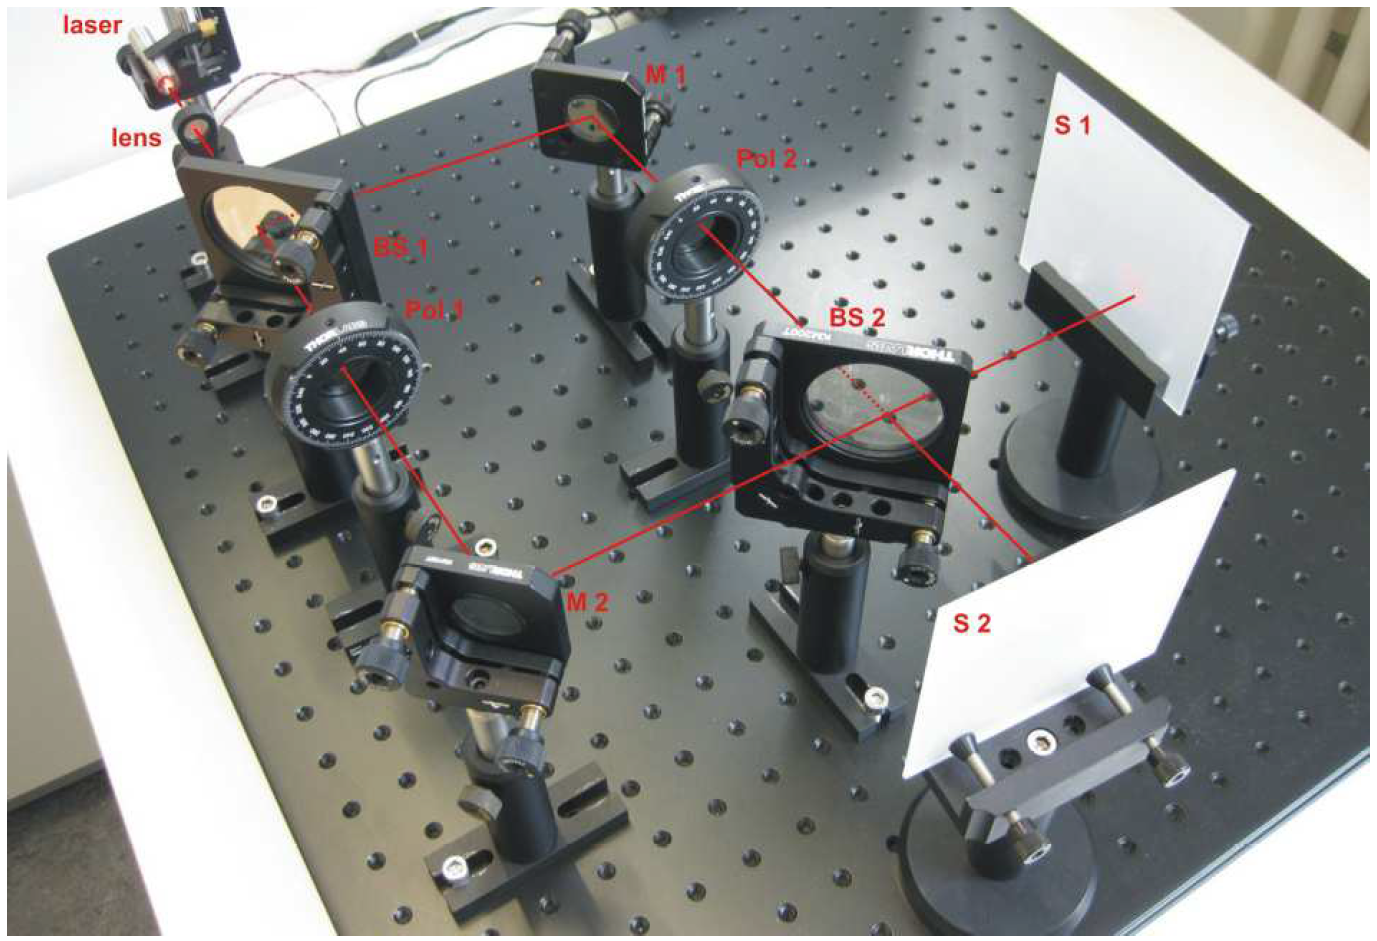
\includegraphics{images/Aufbau.png}
		\caption{Experimenteller Aufbau}
		\label{aufbau}
	\end{center}
\end{figure}

\end{document}
